
\section{Feature set}

\subsection{Motivación}

\begin{frame}
\frametitle{¿Cómo transformar la posición a un vector?}
\begin{figure}
\centering
\includegraphics<1>[width=1.0\linewidth]{../assets/slides/fs_motiv.pdf}
\includegraphics<2>[width=1.0\linewidth]{../assets/slides/fs_motiv2.pdf}
\end{figure}
\end{frame}

\subsection{Definición}

\begin{frame}
\frametitle{Definición}
\begin{figure}
Un \textbf{feature set} $\bm{S_P}$ se define con un conjunto $\bm{S}$ y\\ un predicado asociado $\bm{P(e)}$, donde: \\
\vspace{0.5cm}
\begin{itemize}
    \item $\bm{S}$ es un conjunto de conceptos (rol, color, celda, número, etc.).
    \item $\bm{P(e)}$ es un predicado que determina si $e$ está presente (o \textit{activo}) en la posición (implícita).
    \vskip 0.6cm
    \item<2-> Cada elemento en $S_P$ es un \textit{feature}.
    \item<3-> Cada \textit{feature} es un valor en el vector de entrada, valiendo 1 si está \textit{activo} y 0 si no.
\end{itemize}
\end{figure}
\end{frame}


\begin{frame}
\frametitle{Ejemplos de $S$}
Información posicional:

\begin{center}
\begin{tabular}{cc}

$\begin{aligned}[t]
\featureset{Files} &= \{a, b, ..., h\} \\
\featureset{Ranks} &= \{1, 2, ..., 8\} \\
\featureset{Squares} &= \{a1, a2, ..., h8\}
\end{aligned}$

&

\raisebox{-10ex}{
\chessboard[
    clearboard,
    tinyboard,
    showmover=false,
    pgfstyle={text},
    %text=\fontsize{1.2ex}{1.2ex}\bfseries\sffamily \thepieceindex \stepcounter{pieceindex}, %  \currentwq
    text=\fontsize{1.2ex}{1.2ex}\bfseries\sffamily \currentwq,
    markboard
]
}

\end{tabular}
\end{center}

Información sobre las piezas:

\begin{center}
$\begin{aligned}[t]
\featureset{Roles} &= \text{\{
    \sympawn\ Pawn,
    \symknight\ Knight,
    \symbishop\ Bishop,
    \symrook\ Rook,
    \symqueen\ Queen,
    \symking\ King\}}\textsuperscript{1} \\
\featureset{Colors} &= \text{\{\white\ White, \black\ Black\}}
\end{aligned}$
\end{center}


\end{frame}


\begin{frame}
\frametitle{Ejemplo completo}
\begin{figure}
\centering
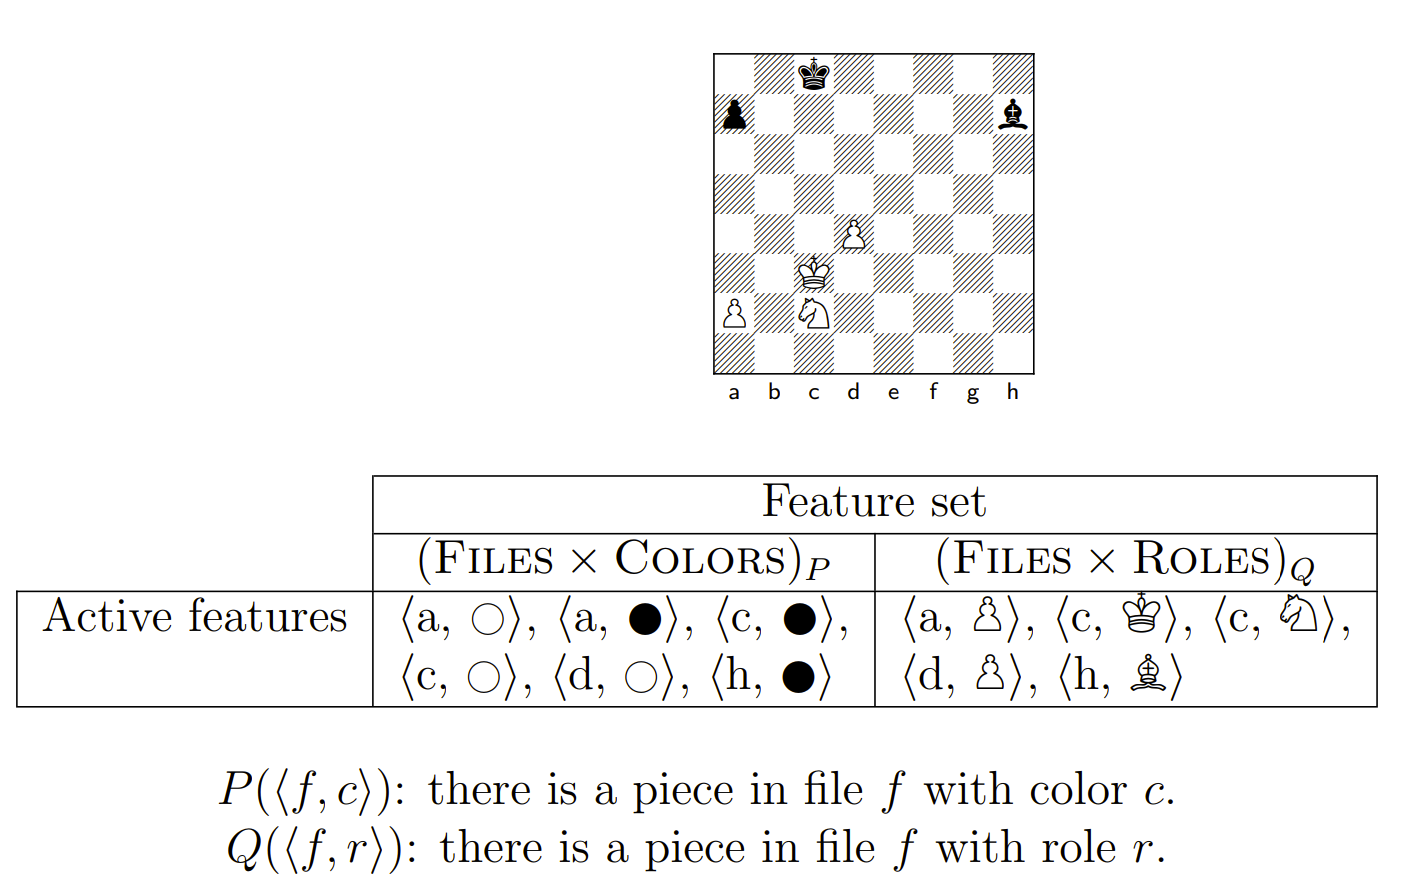
\includegraphics[width=1.0\linewidth]{../assets/slides/fs.png}
\end{figure}
\end{frame}

\subsection{Operadores}

\begin{frame}
\frametitle{Operación: Suma $\oplus$ (concatenación)}
Hay veces que es útil combinar información de dos \textit{feature sets} \\
\pause
\begin{equation*}
S_P, T_Q: \text{feature sets}
\end{equation*}
\begin{equation*}
S_P \oplus T_Q = {(S \cup T)}_R
\end{equation*}
\begin{equation*}
    \text{where } R(e) = \begin{cases}
        P(e) & \text{if } e \in S \\
        Q(e) & \text{if } e \in T
    \end{cases}
\end{equation*}
\end{frame}

\begin{frame}
\frametitle{Operación: Producto $\times$ (and)}
\begin{equation*}
S_P \times T_Q = {(S \times T)}_{R}
\end{equation*}
\begin{equation*}
\text{where } R(\langle e_0, e_1 \rangle) = P(e_0)\ \land\ Q(e_1)
\end{equation*}
\end{frame}

\begin{frame}
\frametitle{Feature set: \featureset{All}}
La codificación más natural de una posición de ajedrez \\
\begin{center}
    $\featureset{All}:\ (\featureset{Squares} \times \featureset{Roles} \times \featureset{Colors})_{P}$ \\
    $P(\langle s, r, c \rangle)$: there is a piece in square $s$ with role $r$ and color $c$\\
\end{center}
\pause
\begin{itemize}
    \item<2-> Es pequeño: $64 \times 6 \times 2 = 768$ \textit{features}
    \item<3-> Es completo: contiene toda la información de la posición
    \item<4-> Es muy rápido computar cuáles \textit{features} están activas
\end{itemize}
\end{frame}

\begin{frame}
\frametitle{Feature set: \featureset{King-All} ó \enquote{KA}}

Los engines modernos usan variaciones del siguiente feature set. Permite entender la posición en relación a la posición del rey:

\begin{center}
    $\featureset{King-All} = \featureset{Square}_{K} \times \featureset{All}$ \\
    $K(s)$: $s$ is the square of the king of the side to move\\
\end{center}

\begin{itemize}
    \item<2-> Es grande: $64 \times 768 = 49152$ \textit{features}
    \item<3-> Es muy rápido como \featureset{All}
    \item<4-> Entrenarlo require un dataset más grande y lleva más tiempo (no me meto acá)
\end{itemize}

\end{frame}
